%%%%%%%%%%%%%%%%%%%%%%%%%%%%%%%%%%%%%%%%%%%%%%%%%%%%%%%%%%%%%%%%%%%%
% Authors: Juan Luis Suárez Díaz
% Tittle: Trabajo de Fin de Grado
% Date: October - 2017
% University of Granada
%%%%%%%%%%%%%%%%%%%%%%%%%%%%%%%%%%%%%%%%%%%%%%%%%%%%%%%%%%%%%%%%%%%%

\documentclass[10pt, compress]{beamer}

\usepackage{spanish}
\usepackage{slides}
\usepackage{mathematics}

\usepackage{booktabs}
\usepackage{comment}
\usepackage{fontawesome}
\usepackage{physics}

\usepackage{multicol}
\usepackage{svg}

% Differential command
\newcommand\diff{\,\mathrm{d}}

% Usual sets notation
\newcommand\C{\mathbb{C}}
\newcommand\R{\mathbb{R}}
\newcommand\Q{\mathbb{Q}}
\newcommand\Z{\mathbb{Z}}
\newcommand\N{\mathbb{N}}

%----------------------------------------------------------------------------------------
%	TITLE, AUTHOR AND OTHER INFO
%----------------------------------------------------------------------------------------

% Title of the document.
\newcommand{\doctitle}{El aprendizaje de métricas de distancia}
% Subtitle.
\newcommand{\docsubtitle}{Análisis y revisión de técnicas desarrolladas en alta dimensionalidad}
% Date.
\newcommand{\docdate}{Septiembre, 2018}
% Subject.
\renewcommand{\subject}{Trabajo de Fin de Grado}
% Author.
\newcommand{\docauthor}{Juan Luis Suárez Díaz}
\newcommand{\docaddress}{Universidad de Granada}
\newcommand{\docemail}{jlsuarezdiaz@correo.ugr.es}
\newcommand{\tutors}{Francisco Herrera Triguero \\ Salvador García López}

\newcommand\itemref[1]{{\renewcommand{\insertenumlabel}{\ref{#1}}%
  \usebeamertemplate{enumerate item}}}

\begin{document}
	
% Title page.

{
	\usebackgroundtemplate{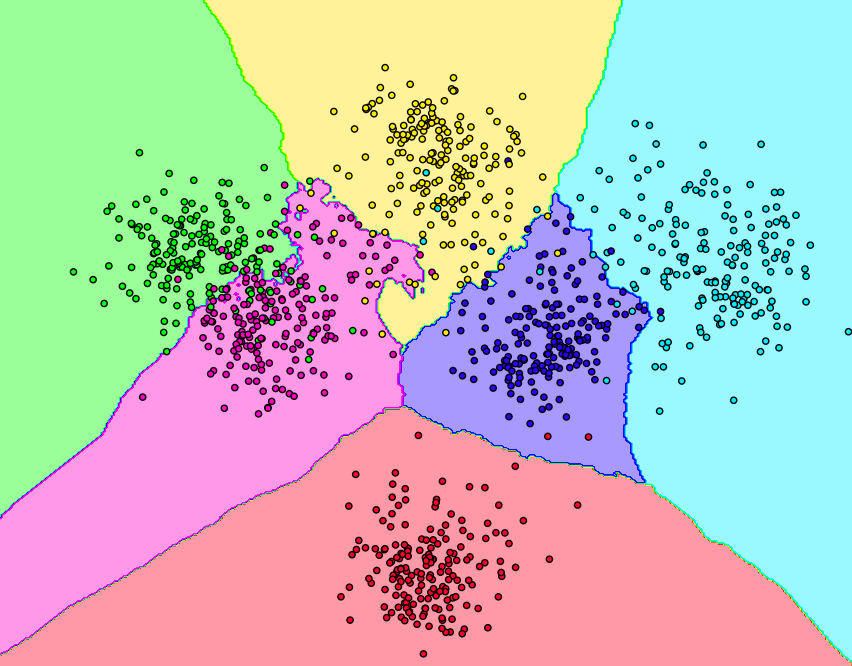
\includegraphics[width=1\paperwidth]{./images/portada.png}}
	\begin{frame}[plain]
		\titlepage
	\end{frame}
}





\section{Introducción}

\subsection{Objetivos}

\begin{frame}{Objetivos}

\begin{itemize}

  \item Conocer la disciplina del aprendizaje de métricas de distancia.

  \item Estudiar los fundamentos matemáticos del aprendizaje de métricas de distancia.

  \item Analizar los principales algoritmos de aprendizaje de métricas de distancia.

  \item Desarrollar un software que integre los algoritmos de aprendizaje estudiados. 

\end{itemize}

\end{frame}


\subsection{Descripción del problema}

\begin{frame}{El aprendizaje de métricas de distancia}

\begin{block}{¿Qué es?}
  Es una rama del aprendizaje automático cuya finalidad es apender distancias a partir de los datos.

\end{block}

\begin{definition}
  Sea $X$ un conjunto no vacío. Una \textbf{distancia} sobre $X$ es una aplicación $d \colon X \times X \to \R$, verificando:
  \begin{enumerate}
    \item $d(x,y) = 0 \iff x = y$ para cualesquiera $x, y \in X$ (coincidencia) \label{item:dist:1}
    \item $d(x,y) = d(y,x)$ para cualesquiera $x, y \in X$ (simetría)
    \item $d(x,z) \le d(x,y) + d(y,z)$ para cualesquiera $x,y,z \in X$ (desigualdad triangular).
  \end{enumerate}
  $\bullet$ \textbf{Pseudodistancias: } Exigen solo $d(x,x) = 0$ en \itemref{item:dist:1}.
\end{definition}

\end{frame}

\begin{frame}{¿Por qué distancias?}
  %\begin{block}{¿Por qué distancias?}
  %  Permiten medir el parecido entre los datos.
  %  \begin{itemize}
  %    \item Datos cercanos $\rightarrow$ Datos similares.
  %    \item Datos lejanos $\rightarrow$ Datos diferentes.
  %  \end{itemize}
  %\end{block}

  \begin{example}{Los clasificadores de vecinos cercanos}
    \centering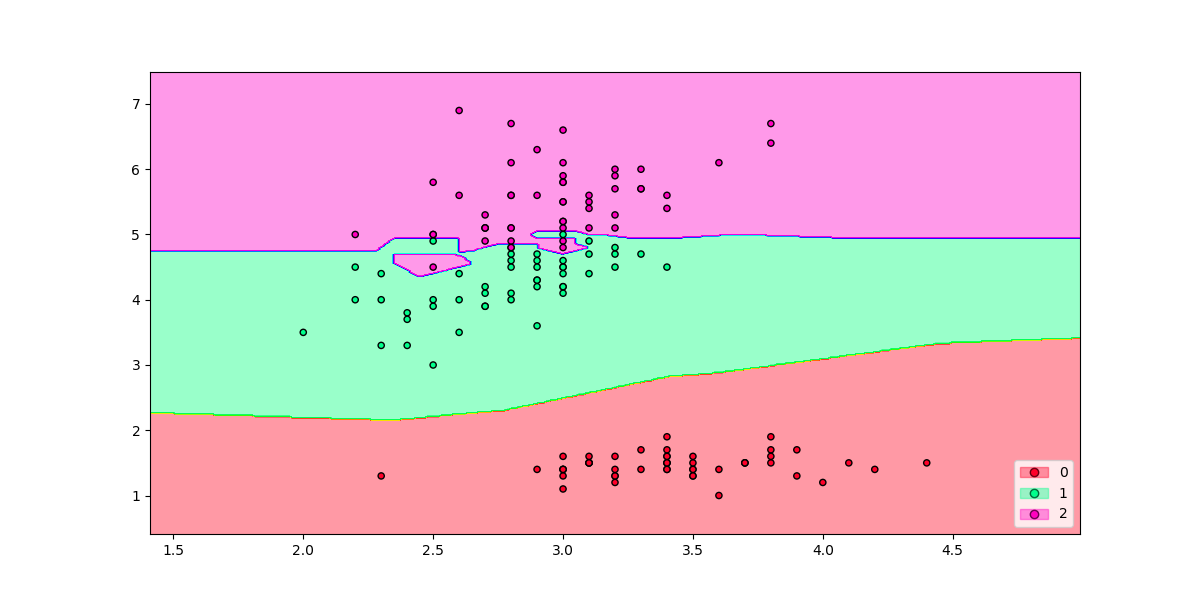
\includegraphics[height=3.5cm]{./images/knn_example.png}
  \end{example}

  \begin{alertblock}{Problema}
    \begin{itemize}
      \item Los algoritmos basados en distancias suelen utilizar distancias fijas.
      \item \textbf{Solución}: Aprender distancias.
    \end{itemize}
  \end{alertblock}
\end{frame}

\begin{frame}{¿Cómo aprender una distancia?}
  \begin{definition}[Distancias de Mahalanobis]
    Sea $M \in \mathcal{M}_d(\R)$ semidefinida positiva. Entonces, $d_M \colon \R^d \times \R^d \to \R$, dada por
    \[ d_M(x,y) = \sqrt{(x-y)^TM(x-y)} \]
    es una (pseudo-)distancia, denominada \textbf{distancia de Mahalanobis}.
  \end{definition}

  \begin{tcolorbox}[colback=ChetwodeBlue!10,colframe=ChetwodeBlue!60]
  \begin{center}
    {\color{TurkishRose} \textbf{Enfoque principal del aprendizaje de métricas de distancia}} \\
    \textbf{Aprender distancias de Mahalanobis sobre espacios vectoriales $d$-dimensionales.}
  \end{center}
  \end{tcolorbox}

  \begin{block}{Dos opciones:}
    \begin{enumerate}
      \item Aprender $M$.
      \item Aprender una aplicación lineal $L$. \\
      Entonces, $M = L^TL$ y $d_M(x,y)^2 = \|L(x-y)\|_2^2$.
    \end{enumerate}
  \end{block}
\end{frame}

\subsection{Aplicaciones}

\begin{frame}{Mejora de clasificadores basados en distancias}
  \centering\includegraphics<1-1>[width=0.75\textwidth]{images/ex_improveknn_1.png}
  \centering\includegraphics<2-2>[width=0.75\textwidth]{images/ex_improveknn_2.png}
  \centering\includegraphics<3-3>[width=0.75\textwidth]{images/ex_improveknn_3.png}
  \centering\includegraphics<4-4>[width=0.75\textwidth]{images/ex_improveknn_4.png}
\end{frame}


\begin{frame}{Organización de datos y reducción de dimensionalidad}
  \centering\includegraphics<1-1>[width=0.75\textwidth]{images/ex_dimred_us_1.png}
  \centering\includegraphics<2-2>[width=0.75\textwidth]{images/ex_dimred_us_2.png}
  \centering\includegraphics<3-3>[width=0.75\textwidth]{images/ex_dimred_us_3.png}
\end{frame}

\section{Matemáticas}


\begin{frame}

  \begin{tcolorbox}[colback=ChetwodeBlue!10,colframe=ChetwodeBlue!60]
    \begin{center}
      {\color{TurkishRose} \small\textbf{Las matemáticas bajo el aprendizaje de métricas de distancia}} \\
      \begin{enumerate}

        \item \textbf{Análisis convexo.} De gran importancia en la mayoría de algoritmos de aprendizaje de métricas de distancia.

        \item \textbf{Análisis matricial.} Las matrices son la herramienta fundamental para modelar el problema.

        \item \textbf{Teoría de la información.} Presente en algunos de los algoritmos.

        \end{enumerate}
    \end{center}
  \end{tcolorbox}

\end{frame}

\subsection{Análisis convexo}

\begin{frame}{Hiperplanos soporte}
  \begin{definition}[Hiperplano soporte]
    Sean $T \colon \R^d \to \R$ lineal, $\alpha \in \R$ y $P = \{x \in \R^d \colon T(x) = \alpha \}$ hiperplano. Definimos $P^+ = \{x \in \R^d \colon T(x) \ge \alpha \}$ y $P^- = \{x \in \R^d \colon T(x) \le \alpha \}$.

    $P$ es un \textbf{hiperplano soporte} para $K \subset \R^d$ si $P \cap \closure{K} \ne \emptyset$ y $K \subset P^+$ o $K \subset P^-$.
  \end{definition}

  \begin{columns}
    \column{0.69\textwidth}
    \begin{theorem}[Teorema del hiperplano soporte]
      \begin{enumerate}
        \item Si $K \subset \R^d$ es convexo y cerrado, para cada $x_0 \in \fr K$ existe un hiperplano soporte $P$ de $K$ tal que $x_0 \in P$.
        \item Todo conjunto convexo cerrado y propio de $\R^d$ es la intersección de todos sus semiespacios soporte.
        \item Sea $K \subset \R^d$ un conjunto cerrado con interior no vacío. Entonces, $K$ es convexo si y solo si para todo $x \in \fr K$ existe un hiperplano soporte $P$ de $K$ con $x \in P$.
      \end{enumerate}
    \end{theorem}

    \column{0.2\textwidth}
    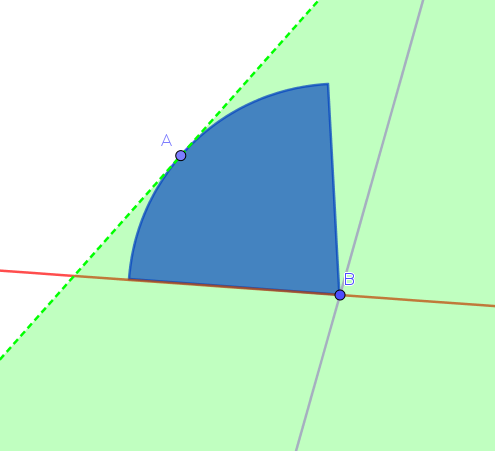
\includegraphics[width=0.9\textwidth]{images/supporting_hyperplane.png}
  \end{columns}
\end{frame}

\begin{frame}{Proyecciones convexas}
  \begin{theorem}[Proyección convexa]
    Si $K \subset \R^d$ es no vacío, cerrado y convexo, entonces, para cada $x \in \R^d$ existe un único punto $P_K(x) \in K$ tal que $d(x,K) = d(x,P_K(x))$: la proyección convexa de $x$ sobre $K$.
  \end{theorem}
  \centering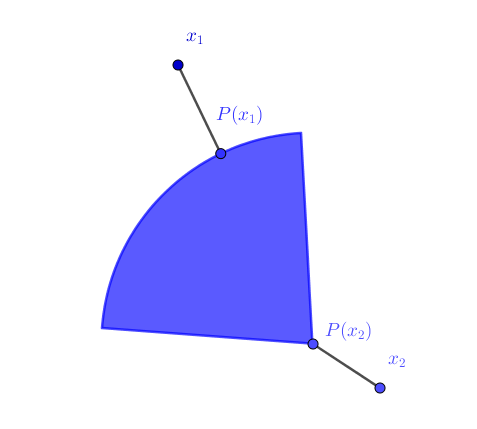
\includegraphics[height=0.5\textheight]{images/convex_projection.png}
\end{frame}

\begin{frame}{Métodos de optimización: gradiente descendente y gradiente con proyecciones}
  \centering\includegraphics<1-1>[width=\textwidth]{images/gradient1_lq.png}
  \centering\includegraphics<2-2>[width=\textwidth]{images/gradient2_lq.png}
  \centering\includegraphics<3-3>[width=\textwidth]{images/gradient3_lq.png}
  \centering\includegraphics<4-4>[width=\textwidth]{images/gradient4_lq.png}
  \centering\includegraphics<5-5>[width=\textwidth]{images/gradient5_lq.png}
\end{frame}

\begin{comment}
\begin{frame}{Método de las proyecciones iteradas}
  \centering\includegraphics<1-1>[width=\textwidth]{images/proyecciones_iteradas1.png}
  \centering\includegraphics<2-2>[width=\textwidth]{images/proyecciones_iteradas2.png}
\end{frame}
\end{comment}

\subsection{Análisis matricial}

\begin{frame}{Matrices como espacio de Hilbert}
  \begin{definition}[Producto escalar y norma de frobenius]
  $A, B \in \mathcal{M}_{d'\times d}(\R)$.
    \begin{align*}
      \langle A, B \rangle_F &= \sum_{i=1}^{d'} \sum_{j=1}^{d} A_{ij}B_{ij} = \tr(A^TB)  \\
      \|A\|_F &= \sqrt{\langle A, A \rangle_F} = \sqrt{\sum_{i=1}^{d'} \sum_{j=1}^{d} A_{ij}^2} = \sqrt{\tr(A^TA)}
    \end{align*}
  \end{definition}

  \begin{equation*}
    \begin{matrix}
      \left(\mathcal{M}_{d' \times d}(\R), \langle \cdot, \cdot \rangle_F\right) & \longleftrightarrow & \left(\R^{d' \times d}, \langle \cdot, \cdot \rangle \right) \\
      & & \\
      \begin{pmatrix}
        a_{11} & \dots & a_{1d} \\
        \vdots & & \vdots \\
        a_{d'1} & \dots & a_{d'd}
      \end{pmatrix} & \longleftrightarrow & (a_{11},\dots,a_{1d}, \dots, a_{d'1},\dots,a_{d'd})
    \end{matrix}
  \end{equation*}
\end{frame}

\begin{frame}[shrink]{Matrices semidefinidas positivas como cono}
  \begin{columns}
  \column{0.66\textwidth}
  \begin{definition}[Cono]
    \begin{itemize}
      \item Un \textbf{cono} es un conjunto $C$ cerrado para combinaciones lineales con coeficientes no negativos.
      \item $C$ es \textbf{sólido} si $\interior{C} \ne \emptyset$.
      \item $C$ es \textbf{puntiagudo} si $C\cap(-C) = \{0\}$.
      \item $C$ es \textbf{propio} si es cerrado, sólido y puntiagudo.
    \end{itemize}

  \end{definition}
  \column{0.21\textwidth}
  \centering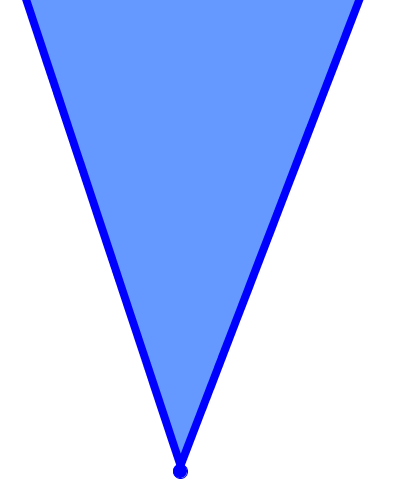
\includegraphics[width=\textwidth]{images/cone.png}

  \end{columns}

  \begin{tcolorbox}[colback=ChetwodeBlue!10,colframe=ChetwodeBlue!60]
    \begin{center}
      {\color{TurkishRose} \small\textbf{El cono de las matrices semidefinidas positivas ($\mathcal{M}_d(\R)^+_0$)}} \\
      Las matrices semidefinidas positivas forman un cono propio sobre el espacio de matrices simétricas, cuyo interior es $\mathcal{M}_d(\R)^+$.
    \end{center}
  \end{tcolorbox}

  \begin{tcolorbox}[colback=ChetwodeBlue!10,colframe=ChetwodeBlue!60]
    \begin{center}
      {\color{TurkishRose} \small\textbf{Orden parcial de matrices como cono propio}}
      \[A, B \in S_d(\R), \quad A \preceq B \iff B - A \in \mathcal{M}_d(\R)^+_0  \]
      \[ \left(\mathcal{M}_d(\R)^+_0 \subset S_d(\R), \preceq \right) \quad \longleftrightarrow \quad \left( \R^+_0 \subset \R , \le \right)\]
    \end{center}
  \end{tcolorbox}

\end{frame}

\begin{frame}[shrink]{Teoremas de descomposición}
  \begin{block}{Conceptos}
    %Conceptos:
    \begin{itemize}
      \item \textbf{Raíz cuadrada: } Dada $M \in \mathcal{M}_d(\R)^+_0$, $\exists^1 N \in \mathcal{M}_d(\R)^+_0 \colon N^2 = M \quad (M^{1/2} := N)$
      \item \textbf{Módulo: } Dada $A \in \mathcal{M}_d(\R)$, $|A| = (A^TA)^{1/2} \in \mathcal{M}_d(\R)^+_0$.
      \item \textbf{Valores singulares: } Dada $A \in \mathcal{M}_d(\R)$, sus valores singulares son los valores propios de $|A|$.
    \end{itemize}
  \end{block}

  \begin{alertblock}{Resultados}
    %Resultados:
    \begin{itemize}
      \item \textbf{Descomposición polar: } $A \in \mathcal{M}_d(\R) \implies \exists U \in O_d(\R) \colon A = U|A|$.
      \item \textbf{Descomposición en valores singulares: } $A \in \mathcal{M}_d(\R) \implies \exists V, W \in O_d(\R) \colon A = W\Sigma V^T$, donde $\Sigma$ es diagonal y contiene los valores singulares de $A$.
      \item \textbf{Descomposición $L^TL$}:
      \begin{enumerate}
        \item $M \in \mathcal{M}_d(\R)^+_0 \iff M = L^TL$, con $L \in \mathcal{M}_d(\R)$.
        \item En tal caso, si $M = K^TK$, entonces $K = UL$, con $U \in O_d(\R)$ ($L$ es única salvo isometrías).
      \end{enumerate}
    \end{itemize}
  \end{alertblock}
\end{frame}

\begin{frame}{Proyección semidefinida}
  \begin{definition}[Parte positiva]
    \begin{enumerate}
      \item Si $D = \diag(\lambda_1,\dots,\lambda_d)$, $D^+ = \diag(\max\{\lambda_1,0\},\dots,\max\{\lambda_d,0\})$.
      \item Si $A \in S_d(\R)$ y $A = UDU^T$, $A^+ = UD^+U^T$.
    \end{enumerate}
  \end{definition}

  \begin{theorem}[Proyección semidefinida]
    Si $A \in S_d(\R)$, $A^+$ es la proyección de $A$ sobre $\mathcal{M}_d(\R)^+_0$.
  \end{theorem}

  \centering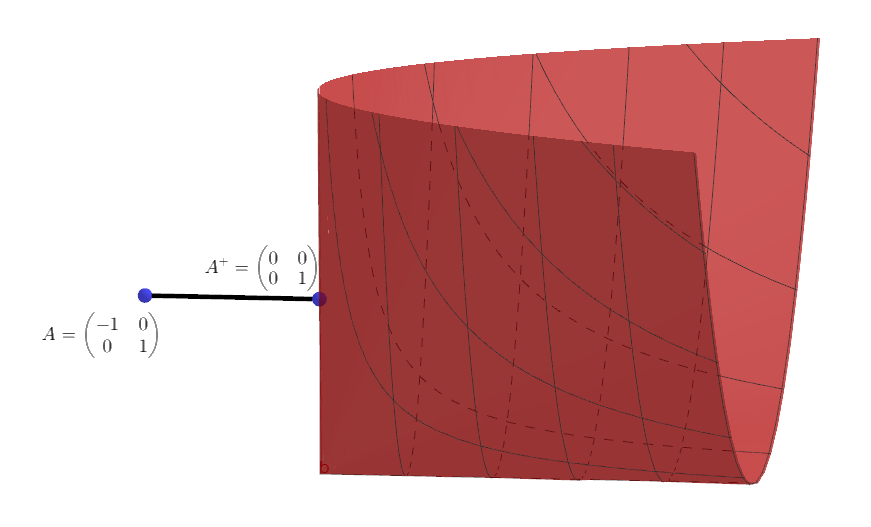
\includegraphics[width=0.5\textwidth]{images/sdp.png}

\end{frame}

\begin{comment}
\begin{frame}{Cociente de Rayleigh}
  \begin{definition}[Cociente de Rayleigh]
    $A \in S_d(\R), \rho_A \colon \R^d \setminus \{0\} \to \R $
    \[ \rho_A(x) = \frac{x^TAx}{x^Tx}\]
  \end{definition}

  \begin{definition}[Cociente de Rayleigh generalizado]
    $ A \in S_d(\R), B \in \mathcal{M}_d(\R)^+, \mathcal{R}_{A.B} \colon \R^d \setminus \{0\} \to \R $
    \[ \mathcal{R}_{A,B}(x) = \frac{x^TAx}{x^TBx}\]
  \end{definition}
\end{frame}
\end{comment}

\begin{frame}[shrink]{Optimización con vectores propios}
  \begin{columns}
  \column{0.49\textwidth}
    \begin{theorem}\label{thm:eigen_trace_opt}
      Sean $d',d \in \N $, con $d' \le d$. Sea $A \in S_d(\R)$, y consideramos el problema de optimización
      
      \begin{equation*}
      \begin{split}
          \max_{L \in \mathcal{M}_{d'\times d}(\R)} &\quad \tr\left(LAL^T\right)  \\
          \text{s.a.: } &\quad LL^T = I.
      \end{split}
      \end{equation*}
      
      Entonces, el problema alcanza un máximo si $L = \begin{pmatrix}
      \text{---} \hspace{-0.2cm} & v_1 & \hspace{-0.2cm} \text{---} \\
      & \dots &  \\
      \text{---} \hspace{-0.2cm} & v_{d'} & \hspace{-0.2cm} \text{---}
      \end{pmatrix}$, donde $v_1,\dots,v_{d'}$ son vectores propios ortonormales de $A$ correspondientes a sus $d'$ mayores valores propios.
      
    \end{theorem}

  \column{0.49\textwidth}

    \begin{theorem} \label{thm:eigen_trace_ratio_opt}
      Sean $d',d \in \N $, con $d' \le d$. Sean $A \in S_d(\R)$ y $B \in \mathcal{M}_d(\R)^+$, y consideramos el problema de optimización
    

      \begin{equation*} \label{eq:eigen_trace_ratio_opt}
      \max_{L \in \mathcal{M}_{d'\times d}(\R)} \quad \tr\left((LBL^T)^{-1}(LAL^T)\right)
      \end{equation*}

      Entonces, el problema alcanza un máximo si $L = \begin{pmatrix}
      \text{---} \hspace{-0.2cm} & v_1 & \hspace{-0.2cm} \text{---} \\
      & \dots &  \\
      \text{---} \hspace{-0.2cm} & v_{d'} & \hspace{-0.2cm} \text{---}
      \end{pmatrix}$, donde $v_1,\dots,v_{d'}$ son los vectores propios de $B^{-1}A$ correspondientes a sus $d'$ mayores valores propios.
    \end{theorem}
  \end{columns}
\end{frame}


\subsection{Teoría de la información}

\begin{frame}{Divergencias}
  \begin{definition}[Divergencia]
    Sea $X$ un conjunto no vacío. Una \textbf{divergencia} es una aplicación $D(\cdot \| \cdot ) \colon X \times X \to \R$ verificando:
    \begin{enumerate}
      \item $D(x \| y ) \ge 0$ para todos $x, y \in X$ (no negatividad).
      \item $D(x \| y ) = 0$ si y solo si $x = y$. 
    \end{enumerate}
  \end{definition}

  \begin{definition}[Divergencia de Kullback-Leibler]
    \[\kl(p \| q) = \mathbb{E}_p\left[ \log\frac{p(X)}{q(X)} \right]\]
  \end{definition}

  \begin{definition}[Divergencia de Jeffrey]
    \[\jf(p \| q) = \kl(p\|q) + \kl(q\|p) \]
  \end{definition}
\end{frame}

\begin{frame}{Algunos resultados}
  \begin{theorem}[Desigualdad de la información]
    $\kl$ es una divergencia.
  \end{theorem}

  \begin{definition}[Divergencia log-det]
    Sean $A, B \in \mathcal{M}_d(\R)^+$.
    \[ D_{ld} (A \| B) = \tr(AB^{-1}) - \log\det(AB^{-1}) - d.\]

  \end{definition}

  \begin{theorem}
    \begin{enumerate}
      \item $D_{ld}$ es una divergencia matricial.
      \item Si $p_1 \sim \mathcal{N}(x|\mu_1,\Sigma_1)$ y $p_2 \sim \mathcal{N}(x|\mu_2,\Sigma_2)$, entonces
      \[ \kl(p_1\|p_2) = \frac{1}{2} D_{ld}(\Sigma_1\|\Sigma_2) + \frac{1}{2}d_{\Sigma_2^{-1}}^2(\mu_1,\mu_2).\]
    \end{enumerate}
  \end{theorem}
\end{frame}

\section{Informática teórica}

\subsection{El aprendizaje de métricas de distancia}

\begin{frame}
  \begin{tcolorbox}[colback=ChetwodeBlue!10,colframe=ChetwodeBlue!60]
    \begin{center}
      {\color{TurkishRose} \small\textbf{Aprendizaje de métricas de distancia}}
      \begin{itemize}
        \item Aprender distancias a partir de los datos.
        \item Dos enfoques: aprender $M$ o aprender $L$.
        \item Mejoran algoritmos de aprendizaje por semejanza y pueden reducir dimensionalidad.
      \end{itemize}
    \end{center}
  \end{tcolorbox}

  \begin{tcolorbox}[colback=ChetwodeBlue!10,colframe=ChetwodeBlue!60]
    \begin{center}
      {\color{TurkishRose} \small\textbf{Algoritmos supervisados: estrategia}}
      \[ \min_{M \in \mathcal{M}_d(\R)^+_0} \ell(d_M, (x_1,y_1), \dots, (x_N, y_N)) \]
    \end{center}
  \end{tcolorbox}
\end{frame}

\subsection{Análisis de algoritmos}

\begin{frame}{Algoritmos estudiados}
  \centering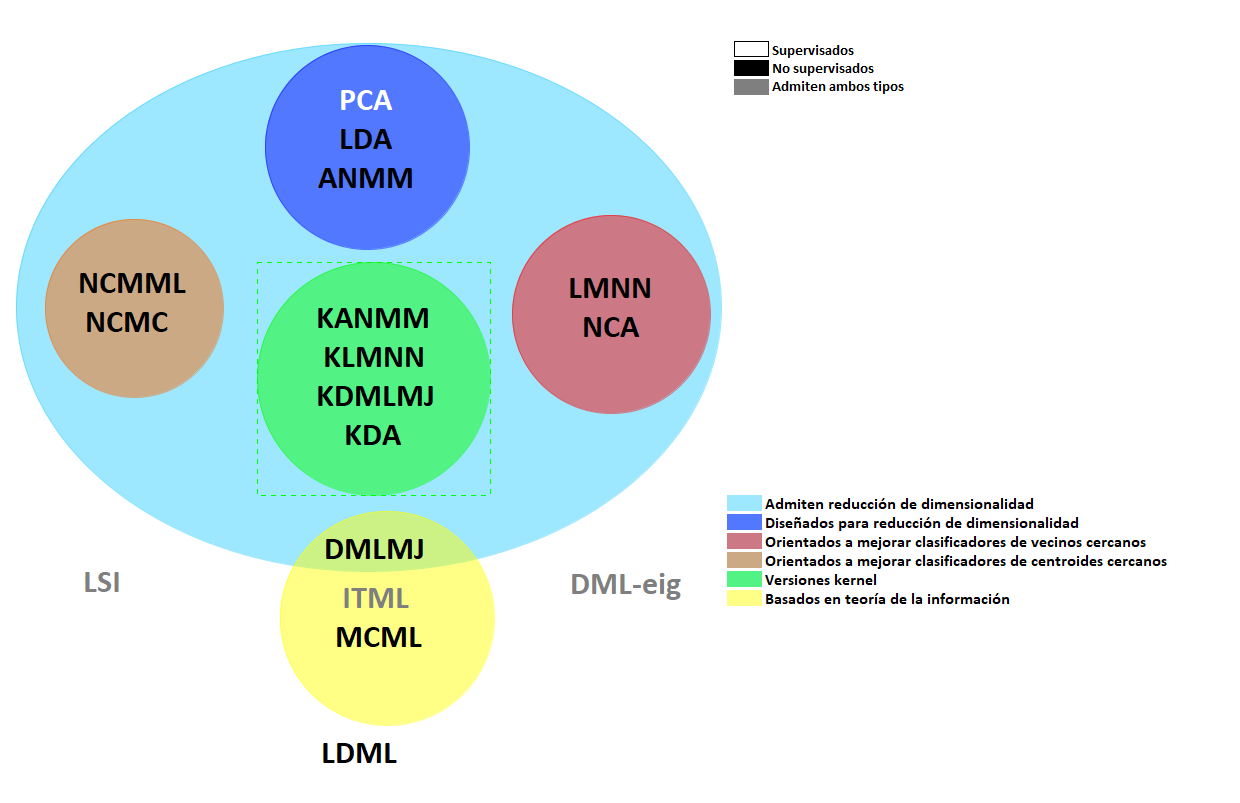
\includegraphics[width=\textwidth]{images/algs.png}
\end{frame}

\begin{frame}[shrink]{Algoritmos centrados en reducción de dimensionalidad}

\begin{minipage}[t][0.4\textheight]{0.45\textwidth}
  \begin{center}\textbf{PCA}\end{center}
  \begin{center}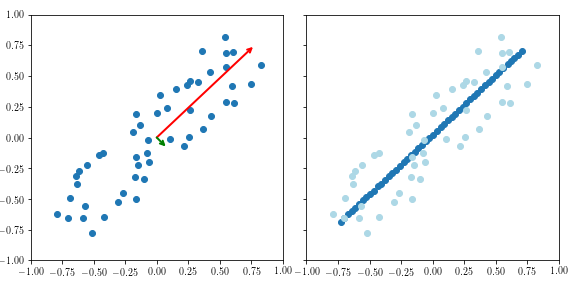
\includegraphics[width=0.9\textwidth]{images/pca1.png}\end{center}
\end{minipage}
\hfill
\begin{minipage}[t][0.4\textheight]{0.45\textwidth}
  \begin{center}\textbf{LDA}\end{center}
  \begin{center}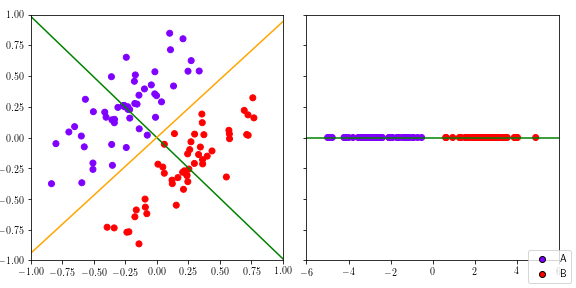
\includegraphics[width=0.9\textwidth]{images/lda.png}\end{center}
  
\end{minipage}

\begin{minipage}[t][0.45\textheight]{0.45\textwidth}
  \begin{center}\textbf{ANMM}\end{center}
  \begin{center}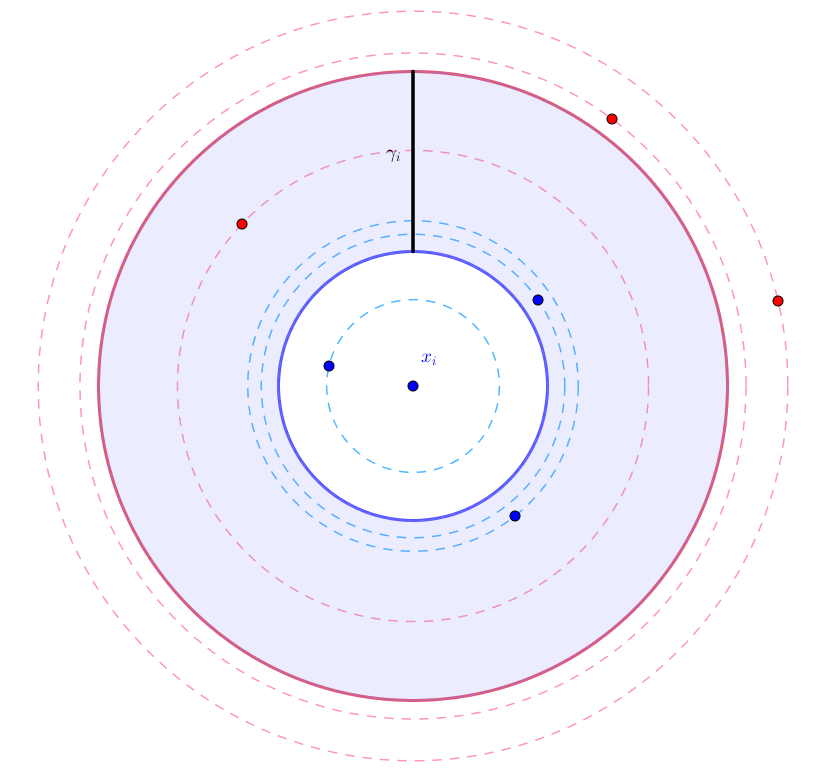
\includegraphics[height=0.7\textwidth]{images/anmm.png}\end{center}
\end{minipage}
\hfill
\begin{minipage}[t][0.45\textheight]{0.45\textwidth}
  \scalebox{.6}{%
  \begin{minipage}[t]{0.9\textwidth}
    \begin{itemize}
      \item \textbf{PCA:} 
            {\begin{equation*}
                \max_{\substack{L \in \mathcal{M}_{d'\times d}(\R) \\LL^T = I}} \quad \tr\left(L \Sigma L^T\right),
            \end{equation*}}
      \item \textbf{LDA:} 
            {\begin{equation*}
            \max_{\substack{L \in \mathcal{M}_{d'\times d}(\R) }} \quad \tr\left((LS_wL^T)^{-1}(L S_b L^T)\right).
            \end{equation*}}
      \item \textbf{ANMM:} 
            {\begin{equation*}
                \max_{\substack{L \in \mathcal{M}_{d'\times d}(\R) \\LL^T = I}} \quad \tr\left(L (S - C) L^T\right),
            \end{equation*}}
      %\scalebox{0.9}{%
      %\begin{minipage}[t]{2.22\textwidth}
      %  \begin{thebibliography}{9}
      %    \setbeamertemplate{bibliography item}[article]
      %    \bibitem{anmm} Fei Wang y Changshui Zhang. “Feature extraction by maximizing the average neighborhood
      %                    margin”. En: Computer Vision and Pattern Recognition, 2007. CVPR’07. IEEE Conference on.
      %                    IEEE. 2007, págs. 1-8.
      %  \end{thebibliography}
      %\end{minipage}
      %}
    \end{itemize}
  \end{minipage}
  }
\end{minipage}

\end{frame}

\begin{frame}{Algoritmos orientados a mejorar el clasificador de vecinos cercanos}

%\begin{columns}

%\column{0.48\textwidth}
\begin{minipage}[t][\textheight][t]{0.48\textwidth}

\begin{center}\textbf{LMNN}\end{center}

\scalebox{.8}{%
\begin{minipage}[t][\textheight][t]{1.25\textwidth}

\textbf{Conceptos:}
\begin{itemize}
  \item \textbf{Target neighbors: } Vecinos que queremos considerar en la clasificación.
  \item \textbf{Impostores: } Invaden el perímetro determinado por los target neighbors.
\end{itemize}

\textbf{Objetivos:}
\begin{itemize}
  \item[\color{ChetwodeBlue}\textbullet] Acercar los target neighbors lo máximo posible.
  \item[\color{ChetwodeBlue}\textbullet] Eliminar los impostores.
\end{itemize}

\fbox{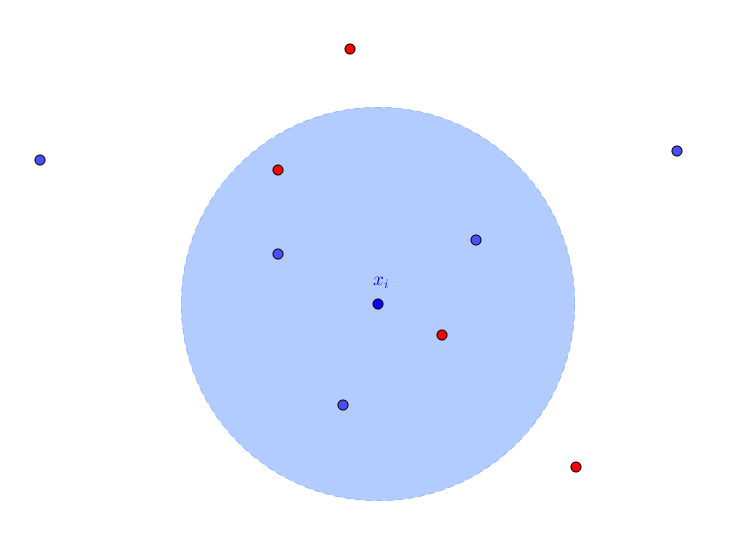
\includegraphics[height=0.3\textwidth]{images/lmnn1.png}}%
\fbox{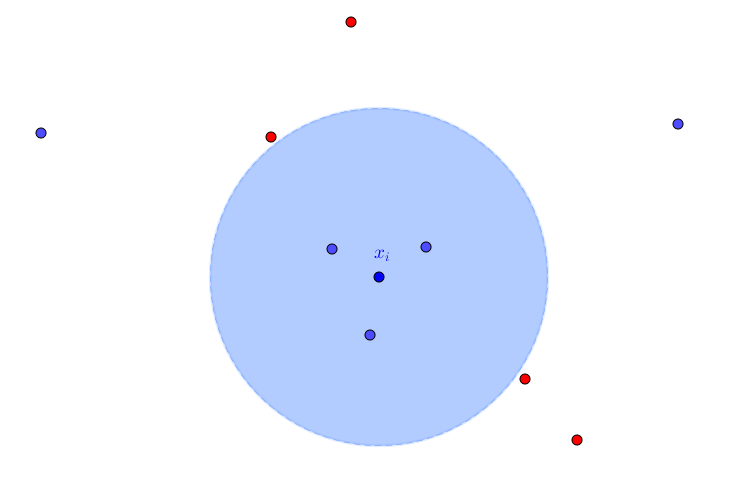
\includegraphics[height=0.3\textwidth]{images/lmnn2.png}}

%\scalebox{1.0}{%
%\begin{minipage}[t]{\textwidth}
%  \begin{thebibliography}{9}
%    \setbeamertemplate{bibliography item}[article]
%    \bibitem{lmnn} Kilian Q Weinberger y Lawrence K Saul. “Distance metric learning for large margin nearest
%                   neighbor classification”. En: Journal of Machine Learning Research 10.Feb (2009), págs. 207-244.
%  \end{thebibliography}
%\end{minipage}
%}

\end{minipage}
}

\end{minipage}
\hfill
\begin{minipage}[t][\textheight][t]{0.48\textwidth}

\begin{center}\textbf{NCA}\end{center}

\scalebox{.8}{%
\begin{minipage}[t][\textheight][t]{1.25\textwidth}

\begin{itemize}
  \item Enfoque probabilístico.
  \item Maximización de la tasa de acierto esperada por la clasificación 1-NN.
  \item Probabilidad de que $x_i$ tenga a $x_j$ como su vecino más cercano:
  \begin{align*} p_{ij}^L &= \frac{\exp(-\|Lx_i - Lx_j\|^2)}{\sum\limits_{k \ne i}\exp(-\|Lx_i - Lx_k\|^2)}\quad (j \ne i),\\
                 p_{ii}^L &= 0
  \end{align*}
  \item Enfoque probabilístico \\$\implies$ Objetivo diferenciable \\$\implies$ Métodos de gradiente \raisebox{-1mm}{
\includegraphics[width=6mm]{./images/blue_tick.png}}
\end{itemize}
%$ $\newline
%\scalebox{1.0}{%
%\begin{minipage}[t]{\textwidth}
%  \begin{thebibliography}{9}
%    \setbeamertemplate{bibliography item}[article]
%    \bibitem{nca} Jacob Goldberger y col. “Neighbourhood components analysis”. En: Advances in neural information
%                   processing systems. 2005, págs. 513-520.
%  \end{thebibliography}
%\end{minipage}
%}

\end{minipage}
}

\end{minipage}
%\end{columns}

\end{frame}

\begin{frame}{Algoritmos orientados a mejorar los clasificadores de centroides cercanos}
  \scalebox{0.6}{%
  \begin{minipage}[t]{1.66\textwidth}
    \begin{block}{Clasificadores basados en centroides}
        Establecen centroides en los datos y clasifican según el centroide más cercano.
    \end{block}
    \begin{exampleblock}{Tipos}
      \begin{enumerate}
        \item \textbf{NCM.} Utiliza las medias de cada clase (\textit{Nearest Class Mean}).
        \item \textbf{NCMC.} Utiliza múltiples centroides por clase, establecidos mediante K-Means.
      \end{enumerate}
    \end{exampleblock}
    \begin{center}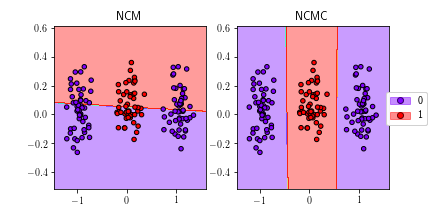
\includegraphics[width=0.35\textwidth]{images/ncm_problem.png}\end{center}
    \begin{alertblock}{Algoritmos de Aprendizaje}
      \begin{itemize}
        \item \textbf{NCMML}, para \textbf{NCM}.
        \item \textbf{NCMC}, para el clasificador \textbf{NCMC}.
        \item Enfoques probabilísticos.
      \end{itemize}
    \end{alertblock}
  \end{minipage}
  }
  %\scalebox{0.6}{%
  %\begin{minipage}[t]{1.66\textwidth}
  %  \begin{thebibliography}{9}
  %    \setbeamertemplate{bibliography item}[article]
  %    \bibitem{ncmml} Thomas Mensink y col. “Metric learning for large scale image classification: Generalizing to new
  %                   classes at near-zero cost”. En: Computer Vision–ECCV 2012. Springer, 2012, págs. 488-501.
  %  \end{thebibliography}
  %\end{minipage}
  %}

\end{frame}

\begin{frame}[shrink]{Algoritmos basados en teoría de la información}
  \begin{block}{Esquema}
    \begin{enumerate}
      \item Fijar una distribución sobre los datos.
      \item Intentar acercar mediante divergencias la distribución a una distribución ``buena''.
      \item Otra opción: alejar distribuciones sobre datos de igual y distinta clase.
    \end{enumerate}
  \end{block}

  \begin{example}[MCML]
    \begin{itemize}
      \item Distribución sobre los datos:
      \[ p^M(j|i) = \frac{\exp(-\|x_i - x_j\|_M^2)}{\sum\limits_{k \ne i}{\exp(-\|x_i - x_k\|^2_M)}}. \]
      \item Distribución ``ideal'':
      \[p_0(j|i) \propto \begin{cases}1, &\quad y_i = y_j \\ 0, &\quad y_i \ne y_j\end{cases}. \]
      \item Problema:
      \[\min_{M \succeq 0}\quad \sum_{i=1}^N \kl \left[ p_0(\cdot|i) \| p^M(\cdot|i) \right]. \]
    \end{itemize}
  \end{example}
\end{frame}

\begin{comment}
\begin{frame}{Algoritmos basados en teoría de la información}
  \begin{minipage}[t][\textheight][t]{0.31\textwidth}

  \begin{center}\textbf{ITML}\end{center}

  \scalebox{.6}{%
  \begin{minipage}[t][\textheight][t]{1.66\textwidth}
    \begin{itemize}
      \item \textbf{Objetivo:} aproximar una métrica inicial satisfaciendo restricciones de similaridad.
      \vspace{8mm}
      \item \textbf{Métrica inicial:} $M_0 \rightarrow p_0 \sim \mathcal{N}(x|\mu, M_0)$.
      \vspace{8mm}
      \item \textbf{Variable: } $M \rightarrow p_M \sim \mathcal{N}(x|\mu,M)$.
      \vspace{8mm}
      \item \textbf{Problema: }
      \begin{equation*} \label{eq:itml:prob1}
        \begin{split}
          \min_{M \succeq 0} &\quad \kl(p_0\|p_M)  \\
          \text{s.a.: } &\quad d_M(x_i,x_j) \le u, \quad (i,j) \in S \\
                        &\quad d_M(x_i,x_j) \ge l, \quad (i,j) \in D.
        \end{split}
      \end{equation*} 
    \end{itemize}
  

  \scalebox{1.0}{%
  \begin{minipage}[t]{\textwidth}
    \begin{thebibliography}{9}
      \setbeamertemplate{bibliography item}[article]
      \bibitem{itml} Jason V Davis y col. “Information-theoretic metric learning”. En: Proceedings of the 24th international conference on Machine learning. ACM. 2007, págs. 209-216.
    \end{thebibliography}
  \end{minipage}
  }

  \end{minipage}
  }

  \end{minipage}
  \hfill
  \begin{minipage}[t][\textheight][t]{0.31\textwidth}

  \begin{center}\textbf{DMLMJ}\end{center}

  \scalebox{.6}{%
  \begin{minipage}[t][\textheight][t]{1.66\textwidth}
  \begin{itemize}
    \item \textbf{Objetivo:} Separar lo máximo posible las distribuciones asociadas a los puntos similares y a los puntos no similares.
    \item \textbf{Vecindarios:} Vecinos más cercanos de igual clase ($V_k^+(x_i) \rightarrow \Sigma_S$) y distinta clase ($V_k^-(x_i) \rightarrow \Sigma_D$).
    \item \textbf{Distribuciones de diferencias:}
    \begin{align*}P_L &\sim \mathcal{N}(x|0,L\Sigma_SL^T)\\ Q_L &\sim \mathcal{N}(x|0,L\Sigma_DL^T).\end{align*}
    \vspace{.3mm}
    \item \textbf{Problema:}
    \[ \max_{L \in \mathcal{M}_{d'\times d}(\R)} \quad  \jf(P_L\|Q_L).\]
  \end{itemize}
  \vspace{.2mm}
  \scalebox{1.0}{%
  \begin{minipage}[t]{\textwidth}
    \begin{thebibliography}{9}
      \setbeamertemplate{bibliography item}[article]
      \bibitem{dmlmj} Bac Nguyen, Carlos Morell y Bernard De Baets. “Supervised distance metric learning through
maximization of the Jeffrey divergence”. En: Pattern Recognition 64 (2017), págs. 215-225.
    \end{thebibliography}
  \end{minipage}
  }

  \end{minipage}
  }

  \end{minipage}
  \hfill
  \begin{minipage}[t][\textheight][t]{0.31\textwidth}

  \begin{center}\textbf{MCML}\end{center}

  \scalebox{.6}{%
  \begin{minipage}[t][\textheight][t]{1.66\textwidth}

  \begin{itemize}
    \item \textbf{Objetivo:} Aproximarse lo máximo posible a la \textit{distribución ideal} donde los puntos de las mismas clases colapsan.
    \item \textbf{Distribución ideal:}
    \[p_0(j|i) \propto \begin{cases}1, &\quad y_i = y_j \\ 0, &\quad y_i \ne y_j\end{cases}. \]
    \item \textbf{Distribución métrica:}
    \[p^{M}(j|i) = \frac{\exp(-\|x_i-x_j\|^2_M)}{\sum\limits_{k\ne i} \exp(-\|x_i-x_k\|^2_M)}.\]
    \item \textbf{Problema:}
    \[\min_{M \succeq 0}\quad \sum_{i=1}^N \kl \left[ p_0(j|i) \| p^M(j|i) \right]. \]
  \end{itemize}

  \scalebox{1.0}{%
  \begin{minipage}[t]{\textwidth}
    \begin{thebibliography}{9}
      \setbeamertemplate{bibliography item}[article]
      \bibitem{mcml} Amir Globerson y Sam T Roweis. “Metric learning by collapsing classes”. En: Advances in neural
                     information processing systems. 2006, págs. 451-458.
    \end{thebibliography}
  \end{minipage}
  }

  \end{minipage}
  }

  \end{minipage}
\end{frame}
\end{comment}

\begin{frame}{Kernel trick y algoritmos basados en kernels}
  \scalebox{0.8}{%
  \begin{minipage}[t]{1.25\textwidth}
  \begin{center}
  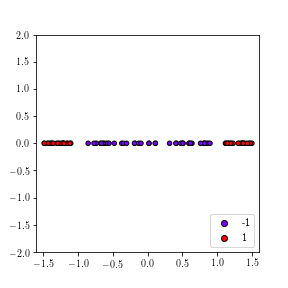
\includegraphics[width=0.2\textwidth]{images/ker_1.png}%
  \raisebox{1.1cm}{
\includegraphics[width=0.05\textwidth]{images/ker_rightarrow2.png}}%
  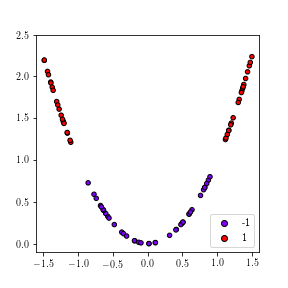
\includegraphics[width=0.2\textwidth]{images/ker_2.png}%
  \raisebox{1.1cm}{
\includegraphics[width=0.05\textwidth]{images/ker_rightarrow2.png}}%
  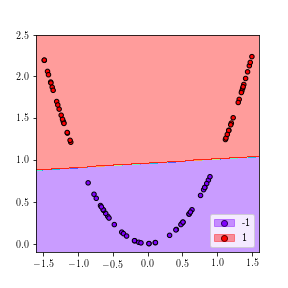
\includegraphics[width=0.2\textwidth]{images/ker_3.png}%
  \raisebox{1.1cm}{
\includegraphics[width=0.05\textwidth]{images/ker_rightarrow2.png}}%
  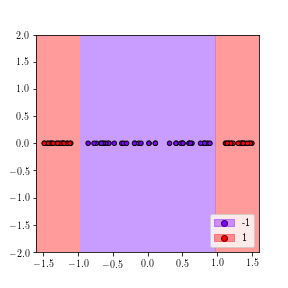
\includegraphics[width=0.2\textwidth]{images/ker_4.png}
  \end{center}
    \begin{block}{Kernel Trick}
      \begin{itemize}
        \item Enviar los datos a un espacio de alta dimensionalidad $\mathcal{F}$, mediante $\phi \colon \R^d \to \mathcal{F}$.
        \item Aprender una distancia en $\mathcal{F}$ mediante $L \colon \mathcal{F} \to \R^{d'}$.
        \item \textbf{Teoremas de representación: } $L\phi(x_i) = AK_{.i}$, con $A$ y $K$ matrices calculables.
        \item \textbf{Ventajas: } Mayor variedad de distancias.
      \end{itemize}
    \end{block}

    \begin{exampleblock}{Algoritmos kernelizados}
      \begin{multicols}{4}
      \begin{enumerate}
        \item KLMNN
        \item KANMM
        \item KDMLMJ
        \item KDA
      \end{enumerate}
      \end{multicols}
    \end{exampleblock}
  \end{minipage}
  }

\end{frame}

\begin{comment}
\begin{frame}{Otros algoritmos}
  \begin{minipage}[t][\textheight][t]{0.28\textwidth}

  \begin{center}\textbf{LSI}\end{center}

  \scalebox{.6}{%
  \begin{minipage}[t][\textheight][t]{1.66\textwidth}
    
    \begin{equation*} \label{eq:lsi:equiv}
    \begin{split}
        \max_{M} &\quad \sum_{(x_i,x_j)\in D}  \|x_i - x_j \|_M \\
        \text{s.a.: } &\quad \sum_{(x_i,x_j) \in S} \|x_i - x_j\|_M^2 \le 1 \\
                      &\quad M \succeq 0.
    \end{split}
    \end{equation*}
  \vspace{0.6cm}

  \scalebox{1.0}{%
  \begin{minipage}[t]{\textwidth}
    \begin{thebibliography}{9}
      \setbeamertemplate{bibliography item}[article]
      \bibitem{itml} Eric P Xing y col. “Distance metric learning with application to clustering with side-information”.
                     En: Advances in neural information processing systems. 2003, págs. 521-528.
    \end{thebibliography}
  \end{minipage}
  }

  \end{minipage}
  }

  \end{minipage}
  \hfill
  \begin{minipage}[t][\textheight][t]{0.28\textwidth}

  \begin{center}\textbf{DML-eig}\end{center}


  \scalebox{.6}{%
  \begin{minipage}[t][\textheight][t]{1.66\textwidth}
  
  \begin{equation*} \label{eq:dmleig:1}
  \begin{split}
      \max_{M} &\quad \min_{(x_i,x_j)\in D}  \|x_i - x_j \|_M^2 \\
      \text{s.a.: } &\quad \sum_{(x_i,x_j) \in S} \|x_i - x_j\|_M^2 \le 1 \\
                    &\quad M \succeq 0.
  \end{split}
  \end{equation*}

  \vspace{1.2cm}
  \scalebox{1.0}{%
  \begin{minipage}[t]{\textwidth}
    \begin{thebibliography}{9}
      \setbeamertemplate{bibliography item}[article]
      \bibitem{dmlmj} Yiming Ying y Peng Li. “Distance metric learning with eigenvalue optimization”. En: Journal of
                      Machine Learning Research 13.Jan (2012), págs. 1-26.
    \end{thebibliography}
  \end{minipage}
  }

  \end{minipage}
  }

  \end{minipage}
  \hfill
  \begin{minipage}[t][\textheight][t]{0.42\textwidth}

  \begin{center}\textbf{LDML}\end{center}

  \scalebox{.6}{%
  \begin{minipage}[t][\textheight][t]{1.66\textwidth}
    \begin{align*}
     \sigma(x) &= \frac{1}{1+e^{-x}}. \\
     p_{ij,M} &= \sigma(b - \|x_i-x_j\|_M^2)\\
     \mathcal{L}(M) &= \sum_{i,j=1}^N y_{ij}\log p_{ij,M} + (1-y_{ij})\log(1-p_{ij,M}) \\
     \max_{M \succeq 0}&\quad \mathcal{L}(M)
   \end{align*}
  
  \scalebox{1.0}{%
  \begin{minipage}[t]{\textwidth}
    \begin{thebibliography}{9}
      \setbeamertemplate{bibliography item}[article]
      \bibitem{mcml} Matthieu Guillaumin, Jakob Verbeek y Cordelia Schmid. “Is that you? Metric learning approaches
                     for face identification”. En: Computer Vision, 2009 IEEE 12th international conference on. IEEE.
                     2009, págs. 498-505.
    \end{thebibliography}
  \end{minipage}
  }

  \end{minipage}
  }

  \end{minipage}
\end{frame}
\end{comment}

\section{Informática práctica}

\subsection{Software desarrollado}

\begin{frame}{Python y R}
  \begin{itemize}
    \item Lenguajes de programación de alto nivel, multiplataforma, orientados a objetos e interpretados.
    \item De gran popularidad en el aprendizaje automático.
    \item Gran cantidad de librerías para computación científica.
    \item Actualmente sin librerías amplias de aprendizaje de métricas de distancia.
  \end{itemize}
  \begin{center}
    
\includegraphics[width=0.3\textwidth]{images/Python.png}
    \hspace{0.2\textwidth}
    
\includegraphics[width=0.3\textwidth]{images/R_logo.png}
  \end{center}
\end{frame}

\begin{frame}
  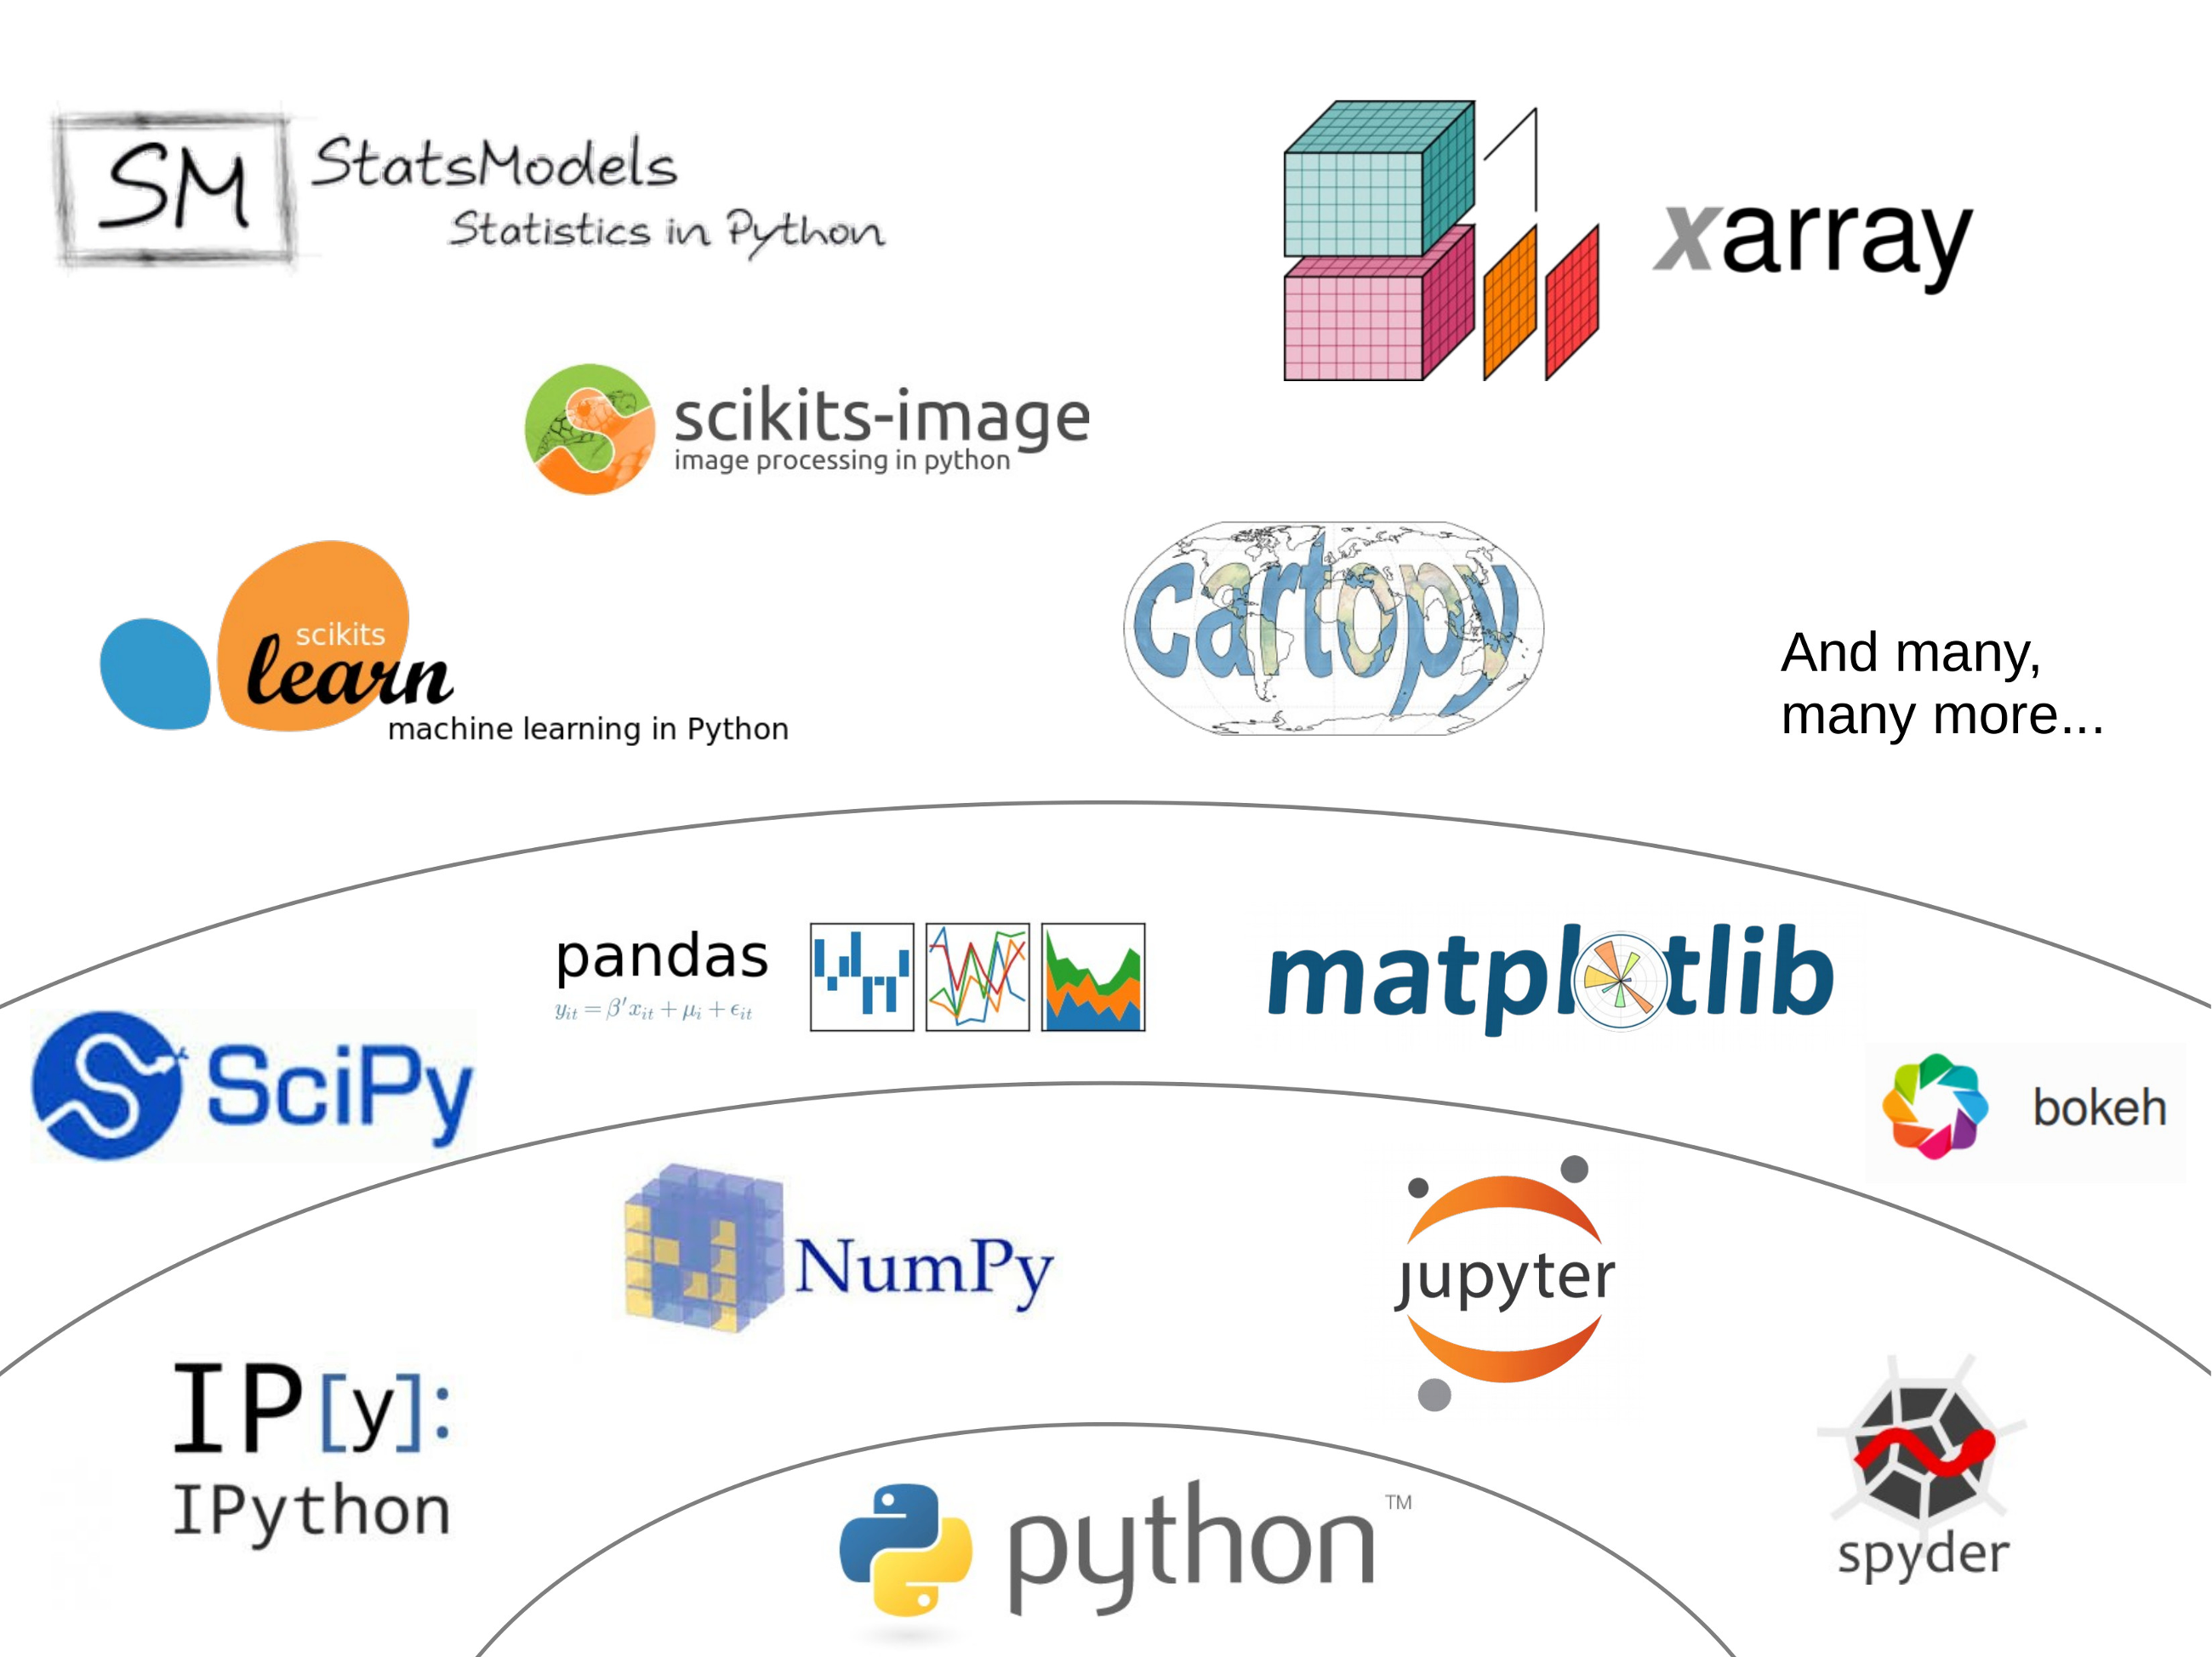
\includegraphics[width=\textwidth]{images/scipy_ecosystem.png}
\end{frame}

\begin{frame}{pyDML}
  \begin{itemize}
    \item \textit{Distance Metric Learning algorithms for Python.}
    \item Incorpora los algoritmos de aprendizaje de métricas de distancia siguiendo la estructura de la librería \textbf{Scikit-Learn}.
    \item Funcionalidades adicionales: clasificadores, dibujo y estimación de parámetros.
  \end{itemize}
  \begin{center}
    
\includegraphics[height=0.15\textheight]{images/github.png}
    \hspace{0.1\textwidth}
    
\includegraphics[height=0.15\textheight]{images/pypi.png}
    \hspace{0.1\textwidth}
    
\includegraphics[height=0.1\textheight]{images/readthedocs.png}
  \end{center}
\end{frame}

\begin{frame}
  \begin{center}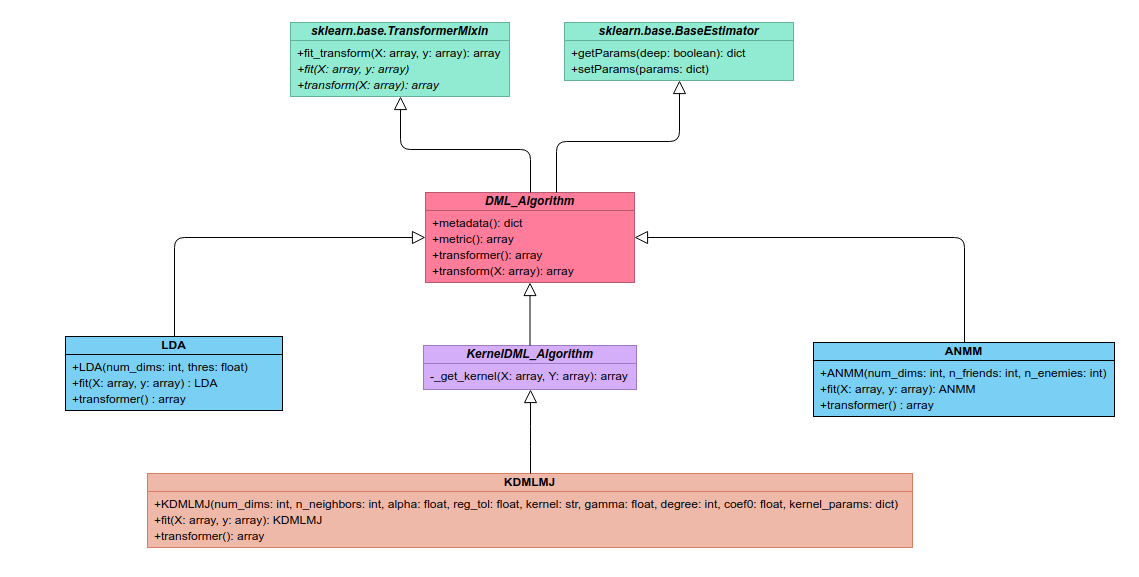
\includegraphics[height=0.5\textheight]{images/uml_pydml.png}\end{center}
  \begin{enumerate}
    \item Construcción: \texttt{alg = LDA(num\_dims = 2)}
    \item Ajuste: \texttt{alg.fit(X,y)}
    \item Resultados del aprendizaje:
      \begin{itemize}
        \item Generalización: \texttt{alg.transform(newX)}
        \item Métrica: \texttt{M = alg.metric()}
        \item Aplicación lineal: \texttt{L = alg.transformer()}
      \end{itemize}
  \end{enumerate}
\end{frame}

\begin{comment}
\begin{frame}{Ejemplo}
  \begin{center}\textbf{Aprendiendo distancias}\end{center}
  \begin{minipage}[t]{0.48\textwidth}
  %\begin{columns}
    %\column{0.5\textwidth}
      \centering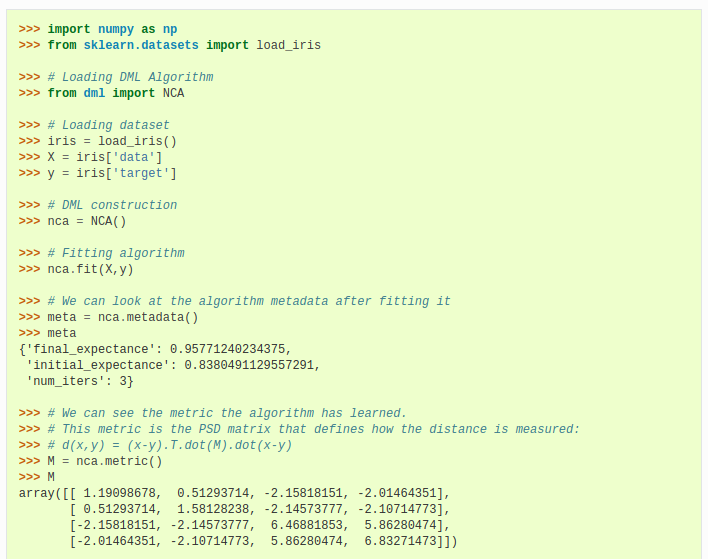
\includegraphics[width=\textwidth]{images/ex_dml1.png}
  \end{minipage}
  \hfill
  \begin{minipage}[t]{0.48\textwidth}
    %\column{0.5\textwidth}
      \centering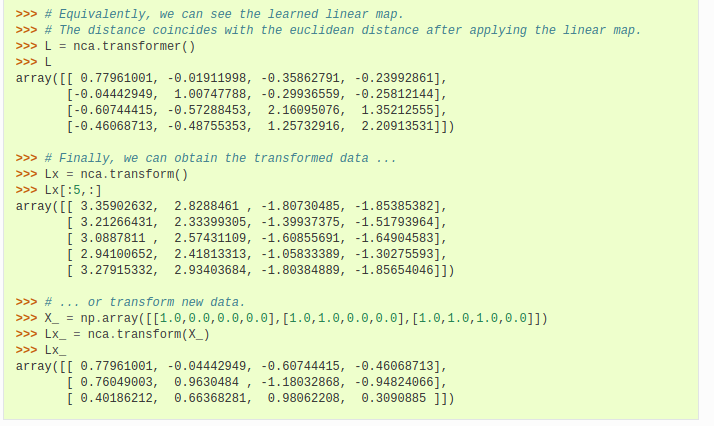
\includegraphics[width=\textwidth]{images/ex_dml2.png}
  %\end{columns}
  \end{minipage}
\end{frame}
\end{comment}

\begin{frame}{Funcionalidades adicionales}
  \begin{center}\textbf{Dibujando regiones de clasificadores basados en distancias} \end{center}
  \centering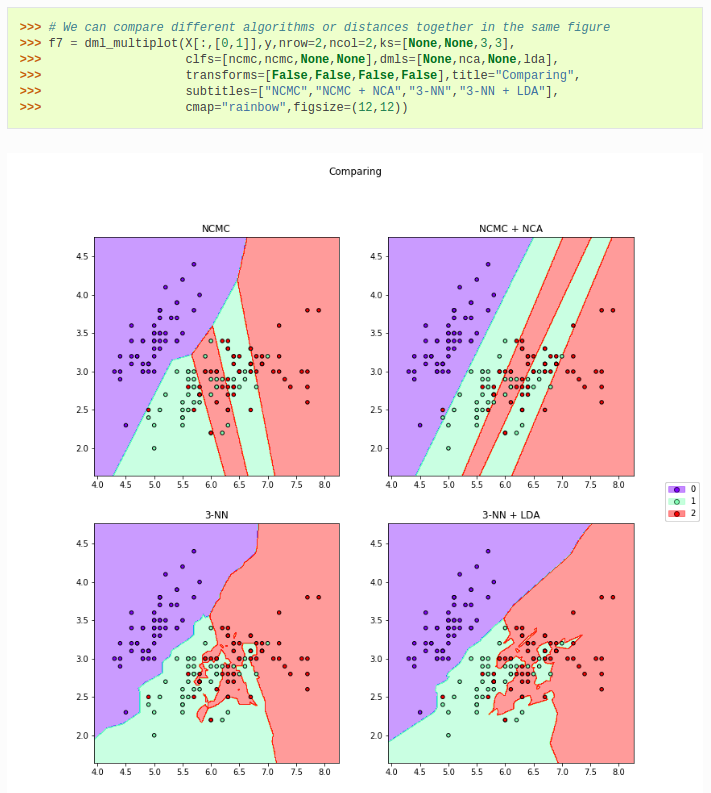
\includegraphics[height=0.8\textheight]{images/ex_plot.png}
\end{frame}

\begin{frame}{Funcionalidades adicionales}
  \begin{minipage}[t]{0.48\textwidth}
  \begin{center}\textbf{Clasificadores basados en distancias}\end{center}
  \begin{center}(Ampliación de los de Scikit-Learn)\end{center}
      \centering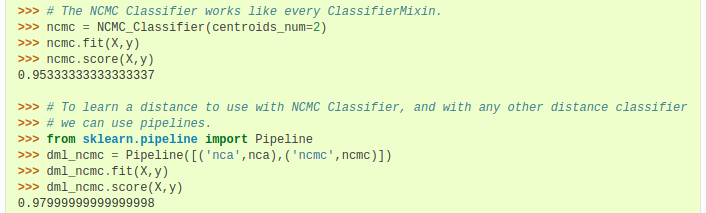
\includegraphics[width=\textwidth]{images/ex_ncmc.png}
  \end{minipage}
  \hfill
  \begin{minipage}[t]{0.48\textwidth}
      \begin{center}\textbf{Estimación de hiperparámetros}\end{center}
      \centering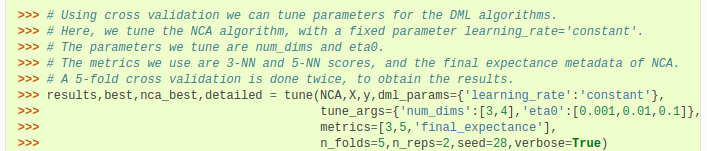
\includegraphics[width=\textwidth]{images/ex_tune1.png}

      \centering
\includegraphics[width=\textwidth]{images/ex_tune2.png}
  \end{minipage}
\end{frame}

\begin{frame}{rDML}
  \begin{itemize}
    \item \textit{Distance Metric Learning algorithms for R.}
    \item Wrapper en R para pyDML.
    \item Pone los algoritmos y funcionalidades adicionales de pyDML a disposición del lenguaje R.
    \item Herramienta de interacción: biblioteca \texttt{reticulate}.
  \end{itemize}

  \begin{center}
    
\includegraphics[height=0.15\textheight]{images/github.png}
    \hspace{0.1\textwidth}
    
\includegraphics[height=0.15\textheight]{images/Rstudio.png}
    \hspace{0.1\textwidth}
    
\includegraphics[height=0.1\textheight]{images/reticulated_python.png}
  \end{center}
\end{frame}

%\begin{frame}{Ejemplo}
%  \begin{center}\textbf{Aprendiendo distancias con rDML}\end{center}
%  \begin{minipage}[t]{0.48\textwidth}
%  %\begin{columns}
%    %\column{0.5\textwidth}
%      \centering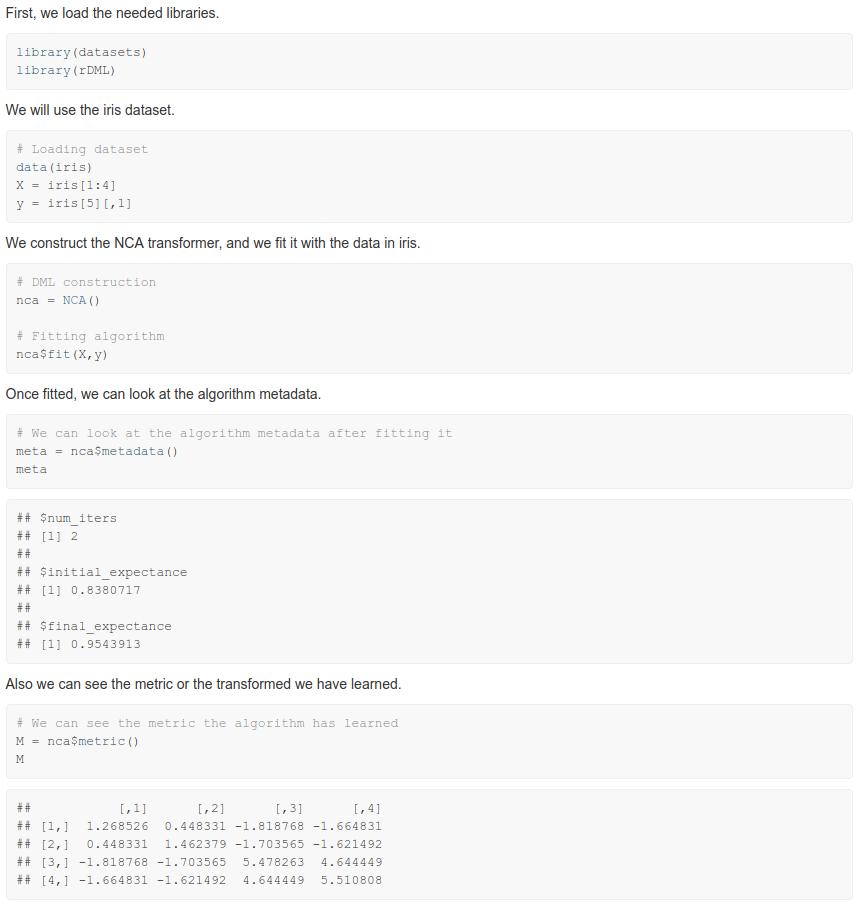
\includegraphics[width=\textwidth]{images/ex_rdml_1.png}
%  \end{minipage}
%  \hfill
%  \begin{minipage}[t]{0.48\textwidth}
%    %\column{0.5\textwidth}
%      \centering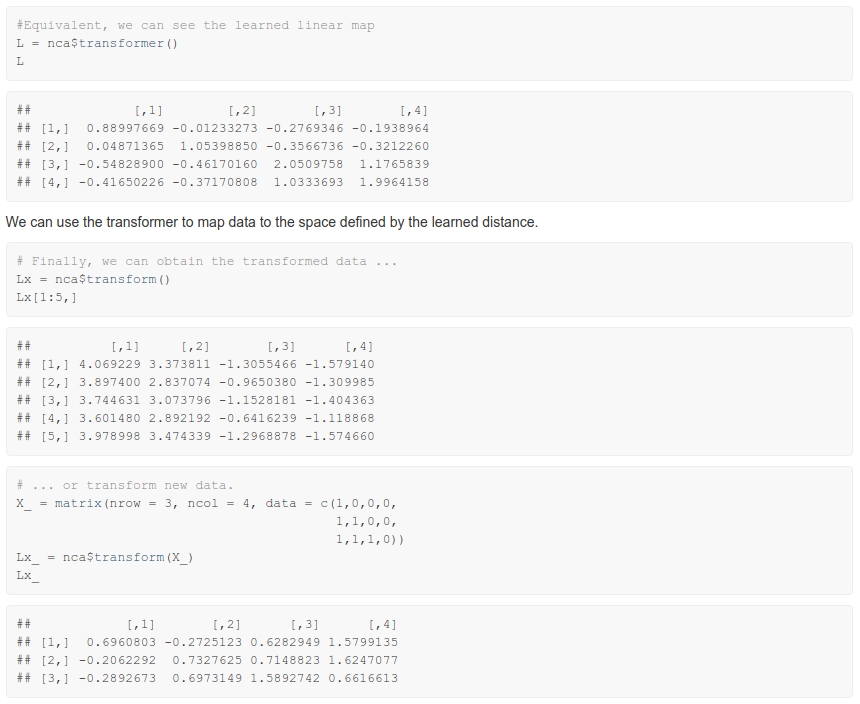
\includegraphics[width=\textwidth]{images/ex_rdml_2.png}
%  %\end{columns}
%  \end{minipage}
%\end{frame}

\subsection{Experimentación}

\begin{frame}[shrink]{Experimentación}
  \begin{alertblock}{Descripción}
    \begin{itemize}
      \item Conjunto de experimentos para evaluar los algoritmos de aprendizaje de métricas de distancia.
      \item Experimentos realizados con la biblioteca pyDML.
      \item Evaluación: resultados de la clasificación con diferentes clasificadores basados en distancias.
      \item 34 datasets.
      \item 10-Fold Cross Validation y normalización previa.
    \end{itemize}
  \end{alertblock} 

  \begin{block}{Experimentos}
    \begin{enumerate}
      \item Algoritmos a dimensión máxima con k-NN.
      \item Algoritmos basados en centroides con sus correspondientes clasificadores.
      \item Algoritmos basados en kernels con k-NN.
      \item Algoritmos de reducción de dimensionalidad con k-NN.
    \end{enumerate}
  \end{block}

\end{frame}

\begin{comment}
\begin{frame}{Algunos resultados}
\resizebox{\textwidth}{!}{%
    \begin{tabular}{lrrrrrrrrrr}
\toprule
{} &  Euclidean &       LDA &      ITML &     DMLMJ &       NCA &      LMNN &       LSI &   DML\_eig &      MCML &      LDML \\
\midrule
appendicitis    &   0.833939 &  0.852273 &  0.860455 &  0.825606 &  0.850455 &  0.842273 &  0.863030 &  0.862273 &  0.851364 &  0.842273 \\
balance         &   0.808237 &  0.899236 &  0.894398 &  0.819113 &  0.958415 &  0.817523 &  0.928073 &  0.894502 &  0.873760 &  0.889554 \\
bupa            &   0.654622 &  0.646555 &  0.628151 &  0.677647 &  0.599412 &  0.634286 &  0.628403 &  0.612017 &  0.574286 &  0.585462 \\
cleveland       &   0.546833 &  0.550267 &  0.552362 &  0.563696 &  0.543678 &  0.580349 &  0.572220 &  0.582941 &  0.578577 &  0.597284 \\
glass           &   0.701514 &  0.623153 &  0.654929 &  0.704158 &  0.691767 &  0.706733 &  0.623567 &  0.626371 &  0.585010 &  0.606334 \\
hepatitis       &   0.832540 &  0.860913 &  0.881548 &  0.889484 &  0.832540 &  0.841865 &  0.913095 &  0.917659 &  0.882937 &  0.854762 \\
ionosphere      &   0.855000 &  0.839472 &  0.886204 &  0.860551 &  0.908431 &  0.885962 &  0.876807 &  0.874118 &  0.863007 &  0.851232 \\
iris            &   0.953333 &  0.953333 &  0.973333 &  0.966667 &  0.966667 &  0.940000 &  0.980000 &  0.960000 &  0.946667 &  0.960000 \\
monk-2          &   0.965537 &  0.956129 &  0.935239 &  0.972460 &  1.000000 &  0.981657 &  1.000000 &  0.990909 &  0.967696 &  0.949577 \\
newthyroid      &   0.953896 &  0.958658 &  0.939827 &  0.944805 &  0.972294 &  0.972511 &  0.963420 &  0.962987 &  0.958225 &  0.967532 \\
sonar           &   0.837013 &  0.778225 &  0.812056 &  0.836147 &  0.870390 &  0.874242 &  0.850671 &  0.797554 &  0.856342 &  0.788680 \\
wine            &   0.960675 &  0.988889 &  0.977376 &  0.966230 &  0.988235 &  0.983299 &  0.966230 &  0.976722 &  0.983299 &  0.988889 \\
movement\_libras &   0.813944 &  0.664214 &  0.799221 &  0.864980 &  0.831939 &  0.802010 &  0.744055 &  0.787242 &  0.807313 &  0.736096 \\
pima            &   0.739662 &  0.752597 &  0.714969 &  0.742259 &  0.737013 &  0.727837 &  0.739576 &  0.726658 &  0.723975 &  0.724009 \\
vehicle         &   0.712582 &  0.762329 &  0.751621 &  0.755180 &  0.755008 &  0.675792 &  0.666690 &  0.650105 &  0.736938 &  0.717077 \\
vowel           &   0.978788 &  0.977778 &  0.953535 &  0.980808 &  0.980808 &  0.977778 &  0.947475 &  0.675758 &  0.873737 &  0.909091 \\
wdbc            &   0.971679 &  0.966446 &  0.966415 &  0.964815 &  0.970079 &  0.963028 &  0.968292 &  0.950717 &  0.964876 &  0.943821 \\
wisconsin       &   0.967859 &  0.967794 &  0.959035 &  0.967859 &  0.964831 &  0.966324 &  0.972206 &  0.970715 &  0.954623 &  0.966346 \\
banana          &   0.855585 &  0.646943 &  0.855603 &  0.856520 &  0.858389 &  0.858300 &  0.851794 &  0.687859 &  0.610209 &  0.631972 \\
digits          &   0.986666 &  0.968319 &  0.972841 &  0.983400 &  0.989427 &  0.986096 &  0.910254 &  0.816843 &  0.968848 &  0.981638 \\
letter          &   0.720827 &  0.796751 &  0.719501 &  0.820461 &  0.861029 &  0.716247 &  0.549663 &  0.321460 &  0.753477 &  0.637251 \\
magic           &   0.805086 &  0.736179 &  0.806144 &  0.807189 &  0.814527 &  0.794554 &  0.792421 &  0.752540 &  0.776673 &  0.695187 \\
optdigits       &   0.977732 &  0.951272 &  0.966963 &  0.976129 &  0.975930 &  0.984048 &  0.930608 &  0.802271 &  0.959112 &  0.959164 \\
page-blocks     &   0.949555 &  0.967908 &  0.961477 &  0.950490 &  0.957739 &  0.943965 &       - &  0.952300 &  0.964205 &  0.940490 \\
phoneme         &   0.799285 &  0.724324 &  0.777087 &  0.800228 &  0.793686 &  0.794612 &  0.766867 &  0.748339 &  0.763283 &  0.711248 \\
ring            &   0.643274 &  0.710104 &  0.735260 &  0.645306 &  0.845951 &  0.661573 &  0.816211 &  0.722303 &  0.822361 &  0.564865 \\
satimage        &   0.856497 &  0.838704 &  0.834163 &  0.864328 &  0.851141 &  0.855846 &  0.846520 &  0.813018 &  0.817149 &  0.550118 \\
segment         &   0.902041 &  0.937075 &  0.926531 &  0.908163 &  0.918707 &  0.892857 &  0.885374 &  0.906803 &  0.931973 &  0.871088 \\
spambase        &   0.865481 &  0.887127 &  0.876682 &  0.852574 &  0.915487 &  0.907075 &  0.911141 &  0.904665 &  0.904758 &  0.898278 \\
texture         &   0.961818 &  0.998182 &  0.975455 &  0.985455 &  0.980000 &  0.921818 &  0.940000 &  0.900909 &  0.974545 &  0.871818 \\
thyroid         &   0.931948 &  0.945086 &  0.940297 &  0.936125 &  0.939569 &  0.931958 &  0.935421 &  0.948568 &  0.932006 &  0.958383 \\
titanic         &   0.758392 &  0.780464 &  0.760933 &  0.758734 &  0.676411 &  0.696411 &      - &  0.733135 &  0.725301 &  0.734112 \\
twonorm         &   0.959500 &  0.975018 &  0.966915 &  0.956122 &  0.979072 &  0.975698 &  0.977045 &  0.981099 &  0.973000 &  0.980424 \\
winequality-red &   0.586563 &  0.573370 &  0.582888 &  0.586076 &  0.576614 &  0.577234 &  0.580989 &  0.529240 &  0.561132 &  0.547197 \\
\bottomrule
\end{tabular}

}
\end{frame}
\end{comment}
    

\begin{frame}{Análisis de resultados}
  \begin{enumerate}
    \item Mejores resultados en clasificación k-NN: \textbf{NCA}, \textbf{LMNN} y \textbf{DMLMJ}.
    \item Buenos resultados de \textbf{NCMML} y \textbf{NCMC} sobre los clasificadores basados en centroides.
    \item Algoritmos basados en kernels: gran variedad de posibilidades.
    \item Ventajas de la reducción de dimensionalidad.
  \end{enumerate}
\end{frame}

\section{Conclusiones y vías futuras}

\subsection{Conclusiones y vías futuras}

\begin{frame}{Conclusiones}
  Hemos estudiado el concepto de aprendizaje de métricas de distancia, con sus fundamentos teóricos y algunos de sus algoritmos. También se han recogido los algoritmos en un software, con el que se han elaborado distintos experimentos.
  \begin{block}{Vías futuras}
    \begin{enumerate}
      \item \textbf{Incorporación de nuevos algoritmos.}
      \item \textbf{Nuevos enfoques para el concepto de distancia.}
      \item \textbf{Kernelización de más algoritmos.}
      \item \textbf{Otros mecanismos de optimización.}
    \end{enumerate}
  \end{block}
\end{frame}






{ \usebackgroundtemplate{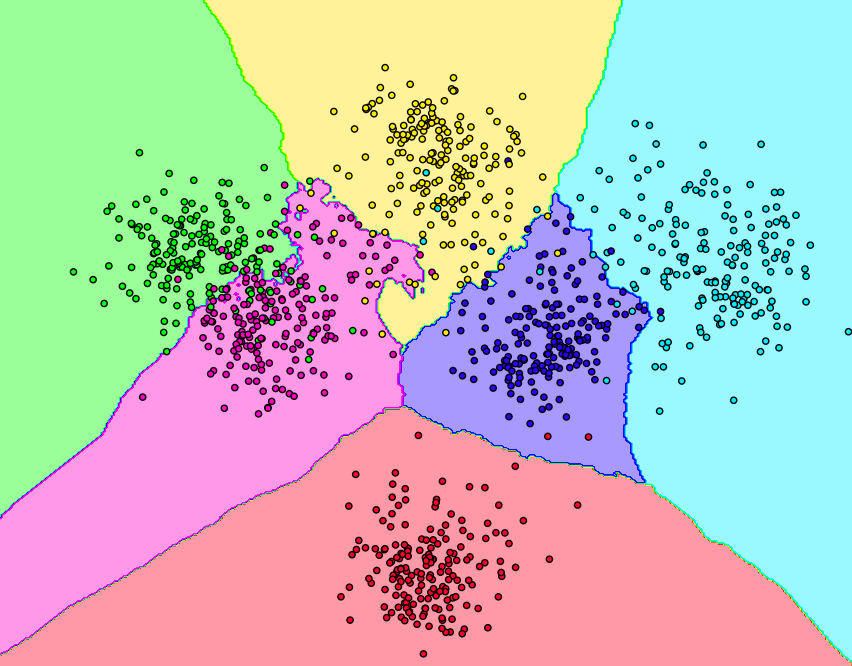
\includegraphics[width=1\paperwidth]{./images/portada.png}}
  \begin{frame}[plain]
    \vspace{0.1\paperheight}
    \begin{titleBox}
      \begin{beamercolorbox}[sep=8pt,center]{title}
        \usebeamerfont{title}\textbf{¡Gracias por su atención!}
      \end{beamercolorbox}

  \begin{beamercolorbox}[sep=8pt,center]{author}  
          \usebeamerfont{author}\large\textbf{\docauthor} \\
          \usebeamerfont{title}\large\docemail
        \end{beamercolorbox}
      \end{titleBox}
    \end{frame}
  }

\end{document}
